\newpage

\chapter{K-Nearest Neighbor}

Most machine learning applications have at least two stages: the learning stage and the deployment stage. 
K-nn is a lazy learner, that is, unlike the decision tree which learns a model (i.e., tree) during the learning stage, it does nothing during the learning stage. 
%
In the deployment stage, it directly computes the result by utilising the information from the training dataset $D$. 
%
While laziness keeps the naive K-nn away from training, it may cause significant computational issues for inference. Every inference takes $O(n)$ time, for $n$ the number of training instances. While linear time in theory, the actual computational time can be significant because $n$ can be large in real-world applications. To tackle this, after the introduction of the basic learning algorithm in Section~\ref{sec:basicknn}, we will introduce methods to speed up K-nn in Section~\ref{sec:speedupknn}. This is followed by a brief discussion regarding how to reasonably output a classification probability as required in many applications, on top of the predictive label. After these, we will present a robustness attack, and discuss other attacks. Unlike the one for decision tree, the robustness attack for K-nn in Section~\ref{sec:robustnessattackknn} utilises constraint solving, and is both sound and complete. 


\section{Basic Learning Algorithm}\label{sec:basicknn}

\begin{definition}
(K-nn) Given a training dataset $D$, a number $k$, a distance measure $||\cdot||$, and a new instance $x$, it is to 
\begin{enumerate}
    \item find $k$ instances in $D$ that are closest to $x$ according to $||\cdot||$, and 
    \item summarise learning result from the labelling information of the $k$ instances, e.g., assign the most occurring label of the $k$ instances to $x$. 
\end{enumerate}
\end{definition}

\subsection*{When to consider?}  Usually, K-nn is useful when there are less than 20 features per instance and we have lots of training data. 
%
Advantages of K-nn include e.g., no training is needed, being able to learn complex target functions, do not lose information, etc. %We will discuss its disadvantages later. 

\subsection*{Classification} Let $(x^{(1)},y^{(1)}), ..., (x^{(k)},y^{(k)})$ be the $k$ nearest neighbors. Formally, the classification is to assign the following label to $x$: 
\begin{equation}\label{equ:knnclass}
    \hat{y} \leftarrow \argmax_{v\in V(Y)}\sum_{i=1}^k \delta(v,y^{(i)})
\end{equation}
where 
\begin{equation}
    \delta(a,b) = \begin{cases}
    1 & \text{if }a = b \\
    0 & \text{otherwise}
    \end{cases}
\end{equation}
Intuitively, it returns the class that has the most number of instances in the $k$ training instances. 

We can also consider its weighted variant, e.g., 
\begin{equation}
    \hat{y} \leftarrow \argmax_{v\in V(Y)}\sum_{i=1}^k w_i\delta(v,y^{(i)})
\end{equation}
where 
\begin{equation}
    w_i = \frac{1}{d(x,x^{(i)})}
\end{equation}
Intuitively, it considers not only the occurrence number of a label but also the quality of those occurrences, i.e., those occurrences that are closer to $x$ has a higher weight.  

\subsection*{Regression} 

For regression task, it is to assign the following value to $x$: 
\begin{equation}
    \hat{y} \leftarrow \frac{1}{k}\sum_{i=1}^k y^{(i)}
\end{equation}
We can also consider its weighted variant, e.g., 
\begin{equation}
    \displaystyle \hat{y} \leftarrow \frac{\sum_{i=1}^k w_iy^{(i)}}{\sum_{i=1}^k w_i}
\end{equation}

\subsection*{Issues} 

The following are a few key issues of K-nn. 
\begin{itemize}
    \item The choice of hyper-parameter $k$. Actually, the increasing of k reduces variance, but increases bias. 
    \item For high-dimensional space, the nearest neighbour may not be close at all. This requires a large dataset when there are many  features. 
    \item Memory-based technique is needed. Naively, it must take a pass through the data for each classification. This can be prohibitive for large data sets. 
\end{itemize}

\subsection*{Irrelevant features in instance-based learning}

In K-nn, the learning can be seriously affected by irrelevant features. For example, an instance may be classified correctly with the existing set of features, but will be classified wrongly after adding a new, noisy feature. 

One way around this limitation is to weight features differently, so that the importance of noise features is reduced. Assume that an instance $x$ is expressed as a function $f(x)=w_0+w_1x_1+...+w_nx_n$, for the instance $x=(x_1,...,x_n)$ of $n$ features. We can find weights $w_i$ by solving the following optimisation problem:  
\begin{equation}
    \argmin_{w_0,...,w_n}\sum_{i=1}^k(f(x^{(i)})-y^{(i)})^2
\end{equation}
Then, we have $f(x)$ as the returned value of the K-nn. 

\section{Speeding up K-nn}\label{sec:speedupknn}

If working with the above naive method, to predict the label for a new point $\textbf{x}\notin D$, K-nn processes the training dataset $D$ during the deployment stage. This requires storing the entire dataset $D$ in the memory and going through all points in $D$. Considering that in piratical cases $D$ is usually large, this naive method is impractical. Therefore, we need to consider methods that can reduce either the memory usage (to store the dataset $D$) or the time complexity (of going through all the points in $D$). 

%There are two general strategies for alleviating this weakness. The first one is to avoid retaining every training instance (edited nearest neighbor) and the second is to use a smart data structure to look up nearest neighbors (e.g. a k-d tree).


\subsection*{Reduction of Memory Usage}


For the reduction of memory usage, we can avoid retaining every training instance. In the following, we introduce the edited nearest neighbor. Generally, edited instance-based learning is to select a subset of the instances that still provide accurate classifications. It can be done through either incremental deletion or incremental growth. Incremental deletion starts with all training data in the memory, and then removes an instance $(x,y)$ if another training instance provides the correct classification for $(x,y)$. Incremental growth starts with an empty memory, and add an instance $(x,y)$ if other training instances in memory do not provide the correct classification for $(x,y)$. 

\subsection*{Reduction of Computational Time through k-d Tree}

For the reduction of computational time, we may consider a smart data structure so that we can quickly look up nearest neighbors without going through all points in $D$. 
%
%First, we discuss techniques to reduce the memory usage of the K-nn algorithm. 
%
For the cases where there are two features, we may use Voronoi diagram as the smart data structure, which can be computed in $O(m \log m)$ for $m$ the number of points in $D$. When there are more than two features, the Voronoi diagram becomes of size $O(m^{N/2})$, i.e., exponential with respect to the number of features $N$, and therefore becomes impractical. 

In the following, we introduce another smart data structure, i.e., k-d tree. A k-d tree is similar to a decision tree except that each internal node 
stores one instance. 
%
%\subsection*{Construction of k-d tree}
First of all, we need to construct a k-d tree for $D$. The construction process proceeds by gradually creating nodes from the root of the tree through 
splitting on the median value of the feature having the highest variance (definition of variance is referred to Section~\ref{sec:variance}). We explain the construction process with the following example. 

\begin{example}\label{example:kdconstruction}
Consider a dataset as in Figure~\ref{fig:kd}. 
\begin{figure}[!htbp]
    \centering
    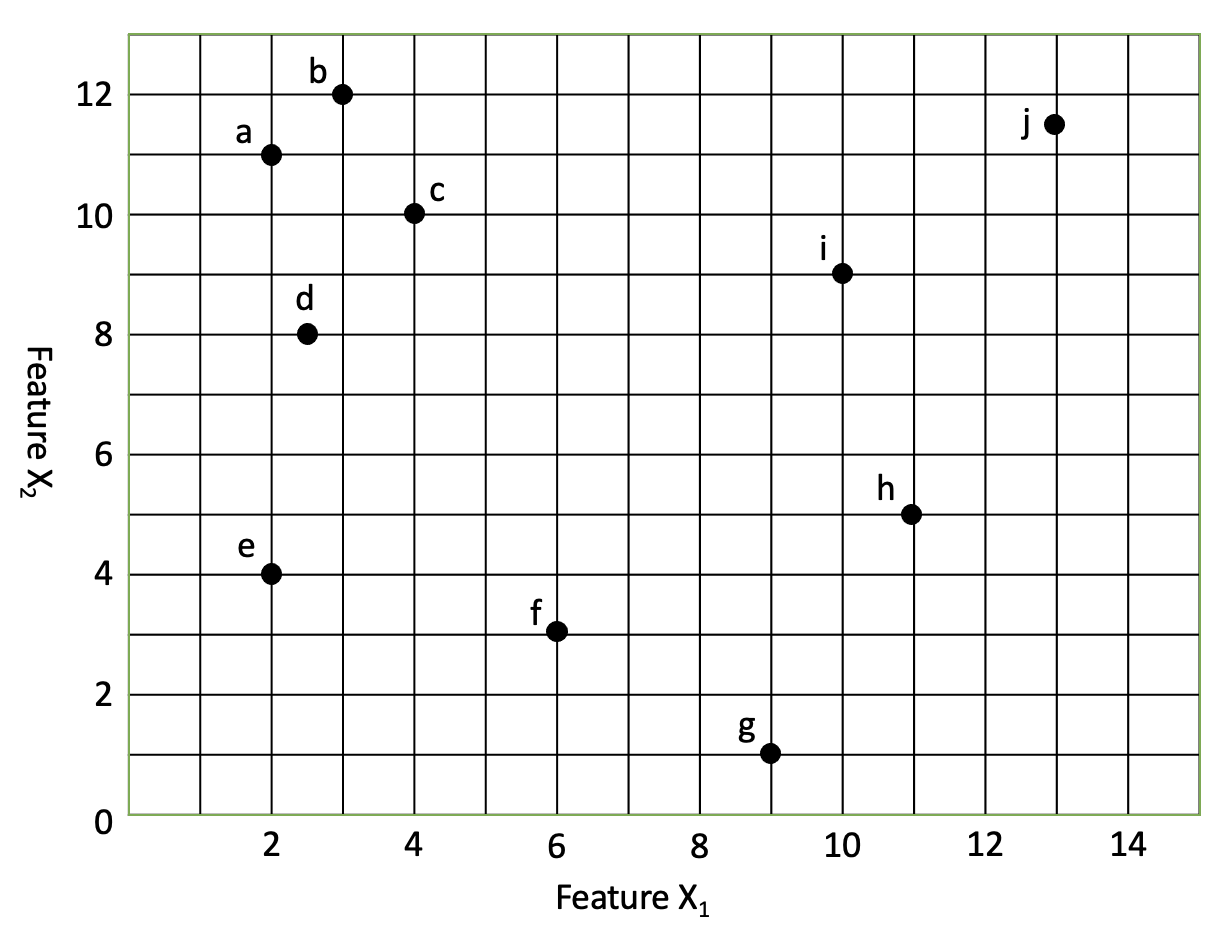
\includegraphics[width=0.7\textwidth]{images/simpleML/kd.png}
    \caption{A simple 2-dimensional dataset}
    \label{fig:kd}
\end{figure}
First of all, we notice that $X_1$-feature (i.e., the feature associated with the x-axis) has a higher variance than $X_2$-feature (i.e., the feature associated with the y-axis). Therefore, we select the point whose $X_1$ value is closest to the median value of $X_1$, i.e., 
\begin{enumerate}
    \item point $f$, with $X_1=6$.
\end{enumerate}
and construct a root node, as shown in Figure~\ref{fig:kd2}(a). 
\begin{figure}[!htbp]
    \centering
    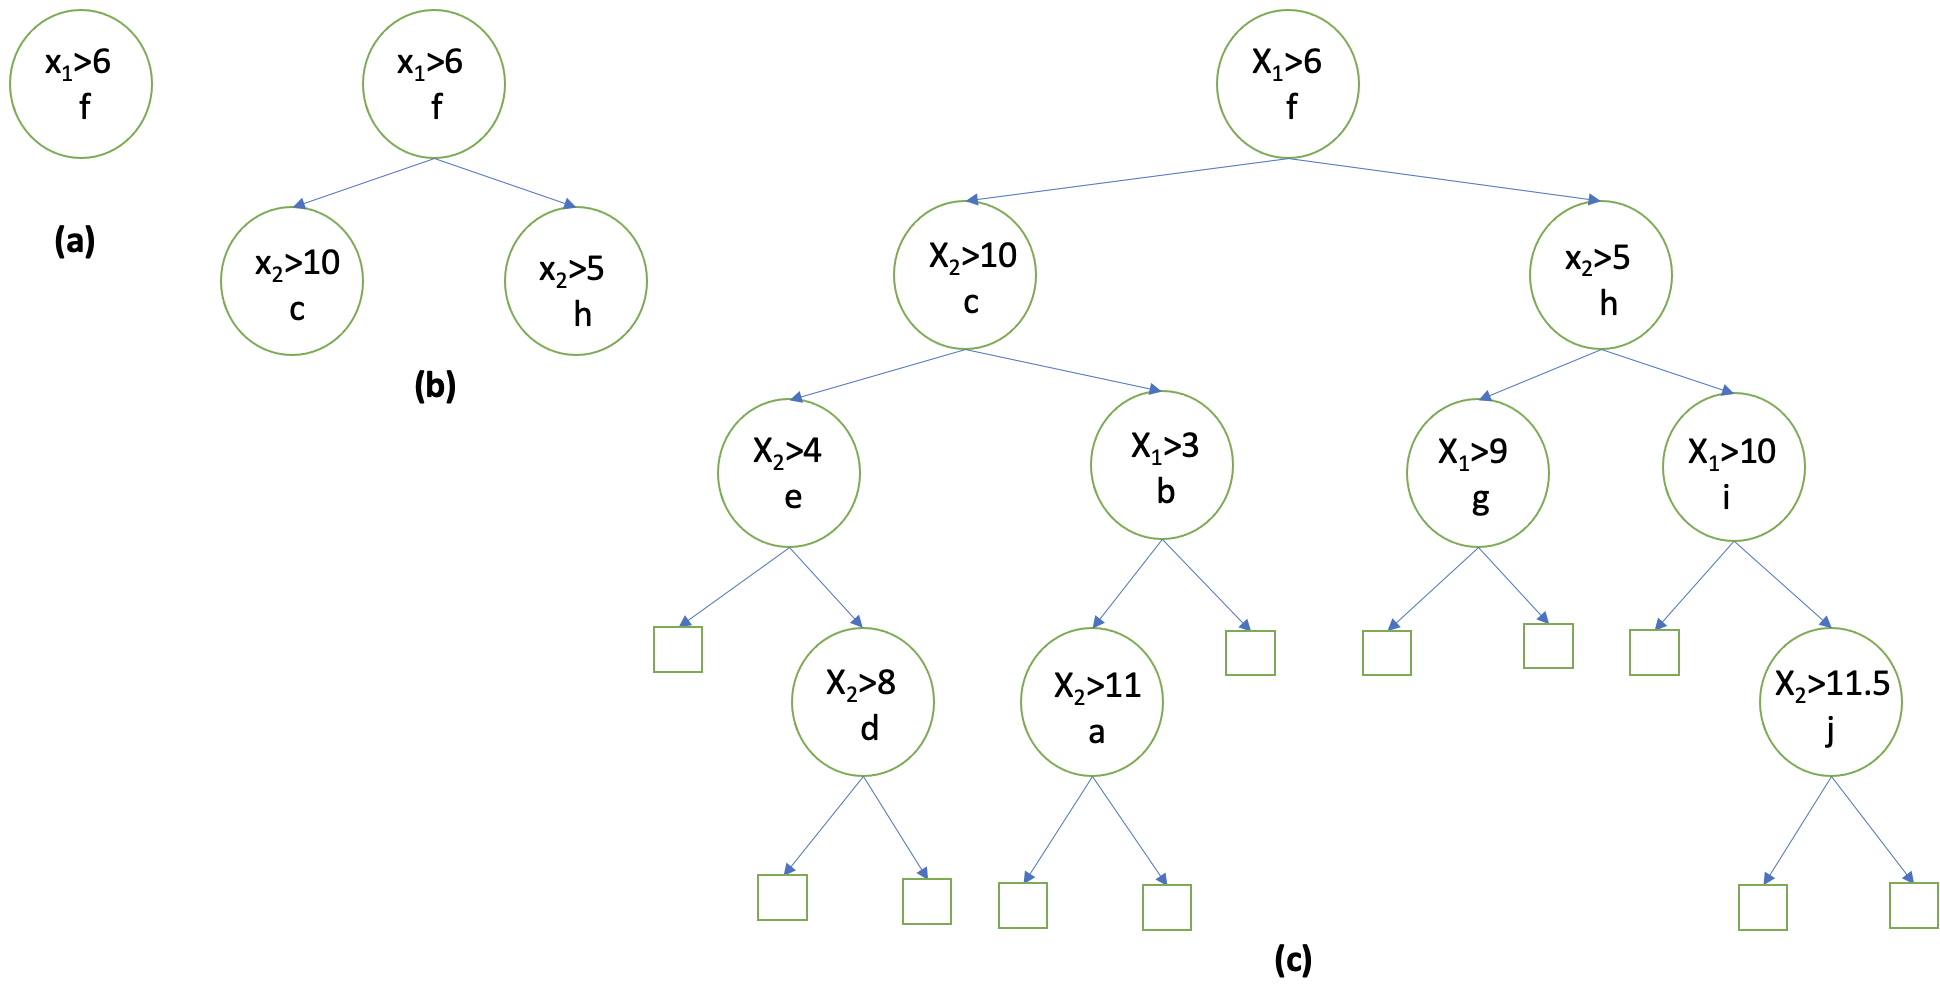
\includegraphics[width=1.0\textwidth]{images/simpleML/kd2.png}
    \caption{Construction of k-d Tree}
    \label{fig:kd2}
\end{figure}
We call $X_1$ the node feature and the number $6$ the node threshold. 
Then, the dataset $D$ can be split into two subsets, with $D_1$ containing those points whose $X_1$ value is no more than $6$ and $D_2$ containing those points whose $X_1$ value is greater than $6$. 

Now, we repeat the above process of ``splitting on the median value of the feature having the highest variance'' on $D_1$ and $D_2$, respectively, and obtain Figure~\ref{fig:kd2}(b) with two more nodes. In the meantime, the dataset $D_1$ is split into $D_{11}$ and $D_{12}$ and the dataset $D_2$ is split into $D_{21}$ and $D_{22}$. 

Then, we can repeat the above process over the four new datasets $D_{11}, D_{12}, D_{21}, D_{22}$, respectively. This process can be repeated and eventually we obtain the k-d tree Figure~\ref{fig:kd2}(c). We create a leaf node when there is an insufficient number of points in the corresponding sub-dataset. 
\end{example}

%\subsection*{Search over k-d Tree}

Once we have a k-d tree, instead of going through all instances for e.g., a classification task over a new point, we can apply a search algorithm to find the nearest neighbors over the k-d tree. Algorithm~\ref{alg:SpeedUpKNN} presents a candidate algorithm. In the following example, we explain the algorithm via an example. 

\begin{example} (Continue with Example~\ref{example:kdconstruction})
Assume that on the k-d tree in  Figure~\ref{fig:kd2}(c), we are to find the nearest neighbour for a new data point $q=(2,3)$. According to Algorithm~\ref{alg:SpeedUpKNN}, we can track the four variables as in the following Table~\ref{tab:kd3} 
\begin{table}[!htbp]
    \centering
    \begin{tabular}{|c|c|c|c|}
    \hline
        distance & best distance & best node & priority queue \\
        \hline
         & $\infty$ && (f,0)\\
         \hline
    \end{tabular}
    \caption{Initialisation of the variables in Algorithm~\ref{alg:SpeedUpKNN}}
    \label{tab:kd3}
\end{table}
which includes their initial values. Then, we pop the priority queue and get $node=f, bound=0$. The execution of one iteration of Line 9-20 will update the variables into the second row of Table~\ref{tab:kd4}. 
\begin{table}[!htbp]
    \centering
    \begin{tabular}{|c|c|c|l|}
    \hline
        distance & best distance & best node & priority queue \\
        \hline
         & $\infty$ && (f,0)\\
         \hline
        4 & 4 & f & (c,0) (h,4)\\
         \hline
    \end{tabular}
    \caption{Values of the variables after the first iteration, in Algorithm~\ref{alg:SpeedUpKNN}}
    \label{tab:kd4}
\end{table}
When popping $(c,0)$ out of the priority queue and get $node=c, bound=0$, we found that $bound  = 0 \not \geq 4 = best~ distance$, which means we need to execute another iteration of Line 9-20. 

The above process repeats. After two more iterations, we get the last row in Table~\ref{tab:kd5}. 
\begin{table}[!htbp]
    \centering
    \begin{tabular}{|c|c|c|l|}
    \hline
        distance & best distance & best node & priority queue \\
        \hline
         & $\infty$ && (f,0)\\
         \hline
        4 & 4 & f & (c,0) (h,4)\\
         \hline
        10 & 4 & f & (e,0) (h,4) (b, 7) \\
         \hline
        1 & 1 & e & (d,1) (h,4) (b, 7) \\
         \hline
    \end{tabular}
    \caption{Values of the variables after the third iteration, in Algorithm~\ref{alg:SpeedUpKNN}}
    \label{tab:kd5}
\end{table}
Now, if  pop out $(d,1)$, we will find that $bound =1 \geq 1 = best~ distance$, and we can terminate the search on Line 7. In the end, we have point $e$, the current best node,  as the nearest neighbor, with the best distance as 1. 
\end{example}

The elements in the priority queue are ordered according to the second element of the pairs. Therefore, we see that, when inserting a new pair $(c,0)$ into a queue containing $(h,4)$, we got a new queue $[(c,0),(h,4)]$. Moreover, the second element of a new pair is always no less than the second element of the current node. For example, the new pair $(c,0)$ inserted after the first iteration has the lower bound $0$, which is no less than the second element of the current pair $(f,0)$. Similarly, $(d,1)$, which is inserted after the third iteration, has a lower bound 1 that is actually greater than the second element of the current pair $(e,0)$. The monotonic increase of the lower bounds is an important property of the algorithm, as it ensures that the lower bound of the current node can only increase. %when starting a new round. 


Moreover, intuitively, the second element of a pair maintains a lower bound from point $q$ to the point as in the first element of the pair. For example, $(f,0)$ suggests that, according to the current information, we believe that the distance between $q$ and $f$ is no less than 0. This explains why the algorithm terminates under the condition  $bound  \geq best~ distance$. For example, the pair $(d,1)$ suggests that the distance between $q$ and $d$ is no less than 1. Since the current best distance is 1 and all the remaining points in the priority queue have a greater lower bound than 1, we can conclude that $d$ is sufficient as the nearest neighbor, according to the monotonicity of the lower bounds as explained earlier. 

\begin{algorithm}[!htbp]
\SetAlgoLined

Queue = \{\}\\
bestDist = $\infty$ \\
Queue.push(root,0) \\
\While{Queue is not empty}{
(node,bound) = Queue.pop()\\
\If{bound $\geq$ bestDist}{
\Return bestNode.instance
}{}{}
dist = distance(x, node.instance)\\
\If{dist $<$ bestDist}{
bestDist = dist \\
bestNode = node
}
\eIf{x[node.feature]-node.threshold > 0}{
Queue.push(node.left, x[node.feature] - node.threshold)\\
Queue.push(node.right, 0)
}{
Queue.push(node.left, 0)\\
Queue.push(node.right, node.threshold - x[node.feature])
}
}
\Return bestNode.instance

 \caption{QueryKdTree($T$, $x$), where $T$ is a k-d tree and $x$ is an instance}
 \label{alg:SpeedUpKNN}
\end{algorithm}





\section{Classification Probability} 

For a classification task, K-nn can only return the label according to Equation (\ref{equ:knnclass}). In cases where the probability of classification is needed, there are ad hoc ways for this purpose. For example, we can let 
\begin{equation}\label{equ:knnprob}
    P(c | \textbf{x}) = \frac{k_c+s}{k+|C|s}
\end{equation}
for all $c\in C$, where $k_c$ is the number of instances in the $k$ neighbors that are with label $c$, and $s$ is a small positive constant that is used to avoid $P(c)=0$ for those classes $c$ that do not appear in the $k$ neighbors. 

Alternatively, let $d_c$ be the average distance from $\textbf{x}$ to the instances with label $c$ in the $k$ neighbors of $\textbf{x}$, we can let  
\begin{equation}\label{equ:knnprob2}
    P(c | \textbf{x}) = \frac{\exp(-d_c)+s}{\sum_{c\in C}\exp(-d_c)+|C|s}
\end{equation}
Note that, we have $d_c=\infty$ (and thus $\exp(-d_c)=0$) if there is no instance of label $c$ in the $k$ neighbors. 

We remark that, the probability $P(c | \textbf{x})$ in Equation (\ref{equ:knnprob}) is actually piece-wise linear over the changing of data instance $\textbf{x}$, because it relies on the number of instances $k_c$. On the other hand, the one in Equation (\ref{equ:knnprob2}) is smoother by considering the average distance $d_c$. 

\section{Robustness and Adversarial Attack} \label{sec:robustnessattackknn}

Given a dataset $D$ of $n$ input samples, and a number $k$, it is not hard to see that the input domain can be partitioned into ${n \choose k}$ disjoint partitions, each of which is determined by $k$ samples such that all inputs in the partition take the $k$ samples as their nearest neighbors. It is noted that, all samples in the same partition share the same predictive label. 
%
Moreover, each partition can be expressed as a finite set of $k(n-k)$ linear (in)equations, each of which expresses that it is closer to one of the $k$ samples than any of the remaining $n-k$ samples. 
%
For any input $\textbf{x}$, we write $R(\textbf{x})$ for the partition it belongs to. Let $\mathcal{R}$ be the set of partitions, and we use $r$ to range over $\mathcal{R}$. 

Now, given an input sample $\textbf{x}$ to be attacked, and any partition $r\neq R(\textbf{x})$, we can define the following optimisation problem to find the input $\textbf{x}'$ that is in partition $r$ and closest to $\textbf{x}$: 
\begin{equation}\label{equ:advexampleknn0}
    closest(\textbf{x},r) = \argmin_{\textbf{x}'\in r} ||\textbf{x} - \textbf{x}'||
\end{equation}
The problem can be solved by applying constraint solver over the above objective with the linear (in)equations of $r$ as constraints. Based on this, the adversarial example can be obtained with the following optimisation problem: 
\begin{equation}\label{equ:advexampleknn}
    r'= \argmin_{r\in \mathcal{R}} [(\textbf{x}'= closest(\textbf{x},r)) \land (y' \neq y)]
\end{equation}
where $y'$ and $y$ are predictive labels of $\textbf{x}'$ and $\textbf{x}$, respectively. Finally, the optimal adversarial example is $closest(\textbf{x},r')$. 

We remark that, the above method is suitable for any classifier that can partition the input domain into a finite number of partitions and each partition can be represented with a finite number of linear (in)equations, such as decision tree and random forest.   


\subsection*{Is $\textbf{x}'$ an adversarial example?}

Yes, the misclassification is ascertained by Equation (\ref{equ:advexampleknn}). 

\subsection*{Is this approach complete?} Yes, the algorithm searches through all partitions (Equation (\ref{equ:advexampleknn})) and all inputs in a partition (Equation (\ref{equ:advexampleknn0})).  

\subsection*{Optimality} The resulting $\textbf{x}'$ is optimal. 


\section{Poisoning Attack}

We can use both the heuristic approaches and the alternating optimisation approach we will introduce in Section~\ref{sec:poisoningattackdeeplearning} for the poisoning attack. Heuristic approaches require the feature extraction function $g$, which is not available for K-nn. However, it can be replaced with the original sample, i.e., let $g(\textbf{x})=\textbf{x}$, because K-nn is mostly working with low- or median-dimensional problems. 

\section{Model Stealing} 

K-nn algorithm does not have a model or trainable parameters. We can use the black-box algorithm that will be introduced in Section~\ref{sec:modelstealingDL} to construct a functionally equivalent model. 


\section{Membership Inference}

An example membership inference attack can be referred to the method in Section~\ref{sec:membershipInferenceDL}. It is  model agnostic and therefore can be applied to any machine learning model.  

\newpage
\section{Practice}


For K-nn, we have the following code to \textbf{simpleML.py} which assumes $k=3$. 

\begin{lstlisting}[language=Python]
from sklearn import datasets
iris = datasets.load_iris()
X_train, X_test, y_train, y_test = train_test_split(iris.data, iris.target, test_size=0.20)
\end{lstlisting}

\begin{lstlisting}[language=Python]
from sklearn.neighbors import KNeighborsClassifier
neigh = KNeighborsClassifier(n_neighbors=3)
neigh.fit(X_train, y_train)
print("Training accuracy is %s"% neigh.score(X_train,y_train))
print("Test accuracy is %s"% neigh.score(X_test,y_test))
\end{lstlisting}


\begin{lstlisting}[language=Python]
print("Labels of all instances:\n%s"%y_test)
y_pred = neigh.predict(X_test)
print("Predictive outputs of all instances:\n%s"%y_pred)

from sklearn.metrics import classification_report, confusion_matrix
print("Confusion Matrix:\n%s"%confusion_matrix(y_test, y_pred))
print("Classification Report:\n%s"%classification_report(y_test, y_pred))
\end{lstlisting}

\begin{lstlisting}[language=Python]
import numpy as np
from math import sqrt
from collections import Counter

# Implement kNN in details
def kNNClassify(K, X_train, y_train, X_predict):
    distances = [sqrt(np.sum((x - X_predict)**2)) for x in X_train]
    sort = np.argsort(distances)
    topK = [y_train[i] for i in sort[:K]]
    votes = Counter(topK)
    y_predict = votes.most_common(1)[0][0]
    return y_predict

def kNN_predict(K, X_train, y_train, X_predict, y_predict):
    acc = 0
    for i in range(len(X_predict)):
        if y_predict[i] == kNNClassify(K, X_train, y_train, X_predict[i]):
            acc += 1
    print(acc/len(X_predict))

print("Training accuracy is ", end='')
kNN_predict(3, X_train, y_train, X_train, y_train)
print("Test accuracy is ", end='')
kNN_predict(3, X_train, y_train, X_test, y_test)
\end{lstlisting}

\begin{lstlisting}[language=Python]
import itertools
import copy 

# Attack on KNN
def kNN_attack(K, X_train, y_train, X_predict, y_predict): 
    m = np.diag([0.5,0.5,0.5,0.5])*4
    flag = True
    for i in range(1,5):
        for ii in list(itertools.combinations([0,1,2,3],i)):
            delta = np.zeros(4)
            for jj in ii:
                delta += m[jj]
                
            if y_predict != kNNClassify(K, X_train, y_train, copy.deepcopy(X_predict)+delta):
                X_predict += delta
                flag = False
                break
                
            if y_predict != kNNClassify(K, X_train, y_train, copy.deepcopy(X_predict)-delta):
                X_predict -= delta
                flag = False
                break
        if not flag:
            break
            
    print('attack data: ',X_predict)
    print('predict label: ',kNNClassify(K, X_train, y_train, X_predict))

X_test_ = X_test[0]
y_test_ = y_test[0]
print('original data: ', X_test_)
print('original label: ', y_test_)
kNN_attack(3, X_train, y_train, X_test_, y_test_)
\end{lstlisting}